% !TEX root = ../main.tex

\section{Простий рух на площині}
Розглянемо найпростіші моделі задач переслідування --- диференціальні ігри на площині з двома учасниками:
переслідувачем $P$ та утікачем $E$, траєкторії яких відповідно позначатимемо $x(t)$ та $y(t)$.
Під \emph{простим рухом} мається на увазі, що закони їх руху описуються системою
\begin{gather}
    \begin{cases}
        \d{x} = u, & \norm{u} \leq \alpha \\
        \d{y} = v, & \norm{v} \leq \beta 
    \end{cases}
\end{gather}
Тут $\norm{z} = \sqrt{z_1^2 + z_2^2}$. Такі закони руху означають, що гравці рухаються з обмеженою швидкістю,
але напрямок руху можуть змінювати довільно. Проінтегрувавши рівняння, можна явно записати траєкторії руху як
\begin{gather*}
    x(t) = x(0) + \intl_0^t u(s) ds, \;
    y(t) = y(0) + \intl_0^t v(s) ds
\end{gather*}
З обмеженості $u$ та $v$ випливає, що 
\begin{gather*}
    \norm{x(t_2) - x(t_1)} \leq \alpha |t_2 - t_1|, \;
    \norm{y(t_2) - y(t_1)} \leq \beta |t_2 - t_1|
\end{gather*}

\begin{example}
    Нехай $u(t) = \begin{pmatrix} -\sin t \\ 2 \cos {2t}\end{pmatrix}$, 
    $v(t) = \begin{pmatrix} -\sqrt{2}\sin t \\ \sqrt{2}\cos t \end{pmatrix}$,
    $x(0) = \begin{pmatrix} 1 \\ 0 \end{pmatrix}$, 
    $y(0) = \begin{pmatrix} \sqrt{2} \\ 0 \end{pmatrix}$, 
    а гра триває до моменту $T = 2\pi$.
    Знайти значення функції виграшу мінімального результату з $H(x, y) = \norm{x - y}$.

    Знайдемо рівняння траєкторій:
    \begin{gather*}
        x(t) = \begin{pmatrix} 1 \\ 0 \end{pmatrix} +
        \intl_0^t \begin{pmatrix} -\sin s \\ 2 \cos {2s} \end{pmatrix} ds = 
        \begin{pmatrix} 1 \\ 0 \end{pmatrix} +
        \l.\begin{pmatrix} \cos s \\ \sin{2s} \end{pmatrix}\r|_0^t = 
        \begin{pmatrix} \cos t \\ \sin{2t} \end{pmatrix}
    \end{gather*}
    \begin{gather*}
        y(t) = \begin{pmatrix} \sqrt{2} \\ 0 \end{pmatrix} +
        \intl_0^t \begin{pmatrix} -\sqrt{2}\sin s \\ \sqrt{2}\cos s  \end{pmatrix} ds = 
        \begin{pmatrix} \sqrt{2}\cos t \\ \sqrt{2}\sin t \end{pmatrix}
    \end{gather*}
    \begin{center}
        \begin{tikzpicture}
        \begin{axis}
            [axis lines = center,
            axis equal,
            trig format plots=rad,
            xmin=-1.5, xmax=1.5, ymin=-1.5, ymax=1.5,
            legend pos = outer north east]
            \addplot [
                domain=0:2*pi,
                samples=100,
                color=red,
                decoration={markings, mark=between positions 0.05 and 0.1 step 2em with {\arrow [scale=1.5]{stealth}}
                }, postaction=decorate, forget plot
            ] ({cos(x)}, {sin(2*x)});
            \addlegendimage{red}
            \addlegendentry{$x(t)$}
            \addplot [
                domain=0:2*pi,
                samples=100,
                color=green,
                decoration={markings, mark=between positions 0.05 and 0.1 step 2em with {\arrow [scale=1.5]{stealth}}
                }, postaction=decorate, forget plot
            ] ({sqrt(2)*cos(x)}, {sqrt(2)*sin(x)});
            \addlegendimage{green}
            \addlegendentry{$y(t)$}
        \end{axis}
    \end{tikzpicture}
    \end{center}
    Значення $K = \underset{0 \leq t \leq 2\pi}{\min} \norm{x(t) - y(t)}$ можна знайти чисельно:
    $K \approx 0.282394$ при $t \approx 0.850448$.
\end{example}

\section{Простий рух в \texorpdfstring{$\R^n$}{Rn}}\label{sec_3_2}
Тепер розглянемо гру переслідування вже не на площині $\R^2$, а в $\R^n$:
\begin{gather}
    \begin{cases}
        \d{x} = u, & \norm{u} \leq \alpha \\
        \d{y} = v, & \norm{v} \leq \beta \\
        x(0) = x_0, \; y(0) = y_0
    \end{cases}
\end{gather}
Тут усі величини є $n$-вимірними векторами, і, як раніше, $x(t)$ --- траєкторія
руху переслідувача $P$, $y(t)$ --- утікача $E$.

Нехай $\alpha > \beta$, тобто, переслідувач може рухатися швидше за утікача. Дослідимо,
чи зможе $P$ наздогнати $E$ та, якщо зможе, як йому потрібно рухатися (за матеріалом в \cite{3}).
Нехай $z = x - y$, тоді маємо систему
\begin{gather*}
    \d{z} = u - v \\
    z(0) = z_0 = x_0 - y_0
\end{gather*}
$P$ може наздогнати $E$, якщо $\exists T < +\infty : z(T) = 0 \Leftrightarrow \norm{z(T)} = 0$.
Введемо функцію $f(t) = \norm{z(t)}^2 = z_1^2(t) + ... + z_n^2(t)$ та дослідимо її похідну.
\begin{gather*}
    \d{f}(t) = 2 z_1(t) \d{z_1}(t) +  ... + 2 z_n(t) \d{z_n}(t) =
    2 \dotprod{z(t)}{\d{z}(t)} = \\ = 2 \l(\dotprod{z(t)}{u(t)} - \dotprod{z(t)}{v(t)} \r)
\end{gather*}
Якщо $u(t) = - \frac{\alpha}{\norm{z(t)}} z(t)$, то 
\begin{gather*}
    \d{f}(t) = 2 \l( -\alpha \norm{z(t)} - \dotprod{z(t)}{v(t)}\r) \leq
    2 \l( -\alpha \norm{z(t)} + \norm{z(t)}\cdot \norm{v(t)}\r) \leq \\
    \leq 2 \l( -\alpha \norm{z(t)} + \beta \norm{z(t)}\r) = 2(\beta - \alpha) \norm{z(t)} = 
    2 (\beta - \alpha) \sqrt{f(t)}
\end{gather*}
Проінтегрувавши від $0$ до $t$ нерівність $\frac{\d{f}(t)}{2\sqrt{f(t)}} \leq \beta - \alpha$,
отримаємо
\begin{gather*}
    \sqrt{f(t)} - \sqrt{f(0)} \leq (\beta - \alpha) t \Leftrightarrow
    \norm{z(t)} - \norm{z(0)} \leq (\beta - \alpha) t \Leftrightarrow \\ \Leftrightarrow
    \norm{z(t)} \leq \norm{z(0)} + (\beta - \alpha) t
\end{gather*}
Оскільки при $t = \frac{\norm{z(0)}}{\alpha - \beta}$ права частина отриманої нерівності дорівнює 0.
Тому, як би не рухався $E$, момент, коли $P$ його наздожене, наступить не пізніше $T(z_0) = \frac{\norm{z_0}}{\alpha - \beta}$.
З іншого боку, якщо $E$ обиратиме $v(t) = -\frac{\beta}{\norm{z(t)}} z(t)$, то
\begin{gather*}
    \d{f}(t) = 2 \l(-\alpha \norm{z(t)} + \beta \norm{z(t)}\r) = 2(\beta - \alpha) \sqrt{f(t)}
\end{gather*}
Інтегруванням отримаємо
\begin{gather*}
    \norm{z(t)} = \norm{z(0)} - (\alpha - \beta) t
\end{gather*}
і тому момент, коли $P$ наздожене $E$, наступить не раніше $T(z_0)$.

Таким чином, яку б стратегію $v(t)$ не обрав утікач $E$, переслідувач $P$ наздожене його не пізніше,
ніж за $\frac{\norm{x_0 - y_0}}{\alpha - \beta}$, використовуючи стратегію $u(t) = - \frac{\alpha}{\norm{x(t) - y(t)}} (x(t) - y(t))$,
причому переслідування буде найдовшим, якщо $E$ обере <<раціональну>> стратегію $v(t) = - \frac{\beta}{\norm{x(t) - y(t)}} (x(t) - y(t))$.

\begin{example}\label{ex_3_2}
    Перевіримо отримані твердження на прикладах. Нехай $n=1$ (переслідування на прямій), $\alpha = 3, \beta = 1$, гра починається з $x_0 = 0$ та $y_0 = 1$ і обидва гравці обирають стратегії, вказані вище.
    Розв'яжемо чисельно (методом Рунге-Кутта) відповідну систему диференціальних рівнянь і подивимося на графіки $x(t)$ та $y(t)$ в залежності від часу.
    Видно, що $P$ дійсно наздогнав $E$ у момент $T = \frac{|0 - 1|}{3 - 1} = 0.5$.
    \begin{center}
        % This file was created by tikzplotlib v0.9.8.
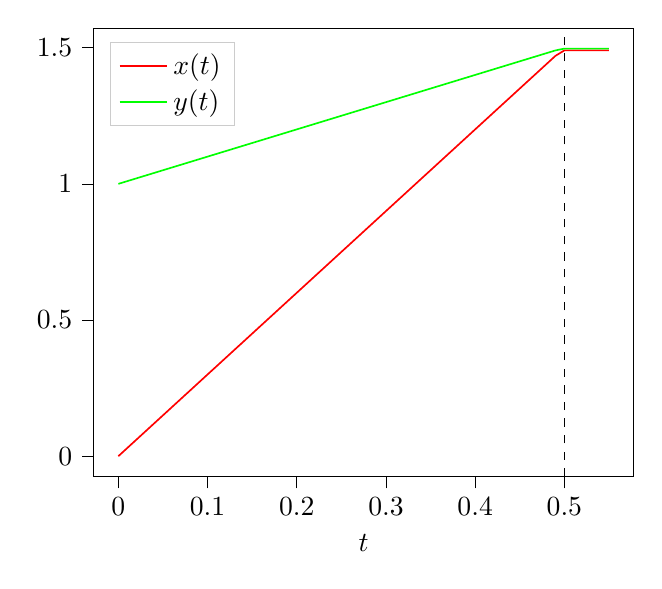
\begin{tikzpicture}

\begin{axis}[
legend cell align={left},
legend style={
  fill opacity=0.8,
  draw opacity=1,
  text opacity=1,
  at={(0.03,0.97)},
  anchor=north west,
  draw=white!80!black
},
tick align=outside,
tick pos=left,
x grid style={white!69.0196078431373!black},
xlabel={\(\displaystyle t\)},
xmin=-0.0275, xmax=0.5775,
xtick style={color=black},
y grid style={white!69.0196078431373!black},
ymin=-0.0748333333333333, ymax=1.5715,
ytick style={color=black}
]
\addplot [semithick, red]
table {%
0 0
0.01 0.03
0.02 0.06
0.03 0.09
0.04 0.12
0.05 0.15
0.06 0.18
0.07 0.21
0.08 0.24
0.09 0.27
0.1 0.3
0.11 0.33
0.12 0.36
0.13 0.39
0.14 0.42
0.15 0.45
0.16 0.48
0.17 0.51
0.18 0.54
0.19 0.57
0.2 0.6
0.21 0.63
0.22 0.66
0.23 0.69
0.24 0.72
0.25 0.75
0.26 0.78
0.27 0.81
0.28 0.840000000000001
0.29 0.870000000000001
0.3 0.900000000000001
0.31 0.930000000000001
0.32 0.960000000000001
0.33 0.990000000000001
0.34 1.02
0.35 1.05
0.36 1.08
0.37 1.11
0.38 1.14
0.39 1.17
0.4 1.2
0.41 1.23
0.42 1.26
0.43 1.29
0.44 1.32
0.45 1.35
0.46 1.38
0.47 1.41
0.48 1.44
0.49 1.47
0.5 1.49
0.51 1.49
0.52 1.49
0.53 1.49
0.54 1.49
0.55 1.49
};
\addlegendentry{$x(t)$}
\addplot [semithick, green]
table {%
0 1
0.01 1.01
0.02 1.02
0.03 1.03
0.04 1.04
0.05 1.05
0.06 1.06
0.07 1.07
0.08 1.08
0.09 1.09
0.1 1.1
0.11 1.11
0.12 1.12
0.13 1.13
0.14 1.14
0.15 1.15
0.16 1.16
0.17 1.17
0.18 1.18
0.19 1.19
0.2 1.2
0.21 1.21
0.22 1.22
0.23 1.23
0.24 1.24
0.25 1.25
0.26 1.26
0.27 1.27
0.28 1.28
0.29 1.29
0.3 1.3
0.31 1.31
0.32 1.32
0.33 1.33
0.34 1.34
0.35 1.35
0.36 1.36
0.37 1.37
0.38 1.38
0.39 1.39
0.4 1.4
0.41 1.41
0.42 1.42
0.43 1.43
0.44 1.44
0.45 1.45
0.46 1.46
0.47 1.47
0.48 1.48
0.49 1.49
0.5 1.49666666666667
0.51 1.49666666666667
0.52 1.49666666666667
0.53 1.49666666666667
0.54 1.49666666666667
0.55 1.49666666666667
};
\addlegendentry{$y(t)$}
\addplot [semithick, black, dashed, forget plot]
table {%
0.5 -0.0748333333333334
0.5 1.5715
};
\end{axis}

\end{tikzpicture}

    \end{center}

    Нехай тепер переслідування відбувається на площині ($n=2$), обмеження швидкостей ті ж самі, гра починається з $x_0 = \begin{pmatrix}
        0 \\ 0
    \end{pmatrix}$ та $y_0 = \begin{pmatrix}
        1 \\ 1
    \end{pmatrix}$.
    \begin{center}
        % This file was created by tikzplotlib v0.9.8.
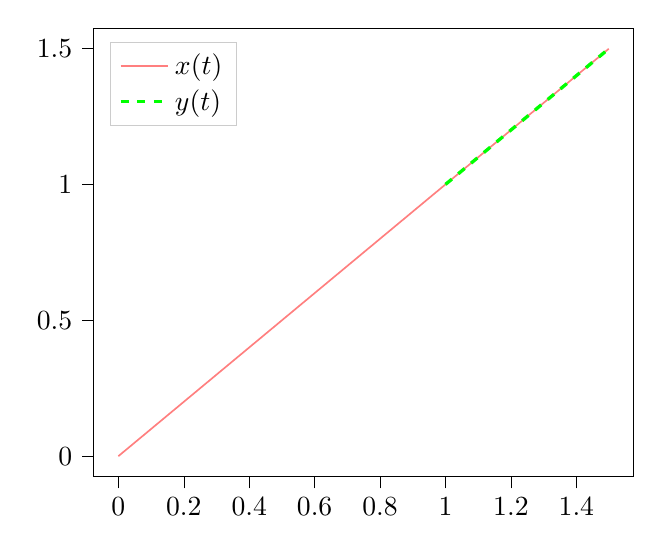
\begin{tikzpicture}

\begin{axis}[
legend cell align={left},
legend style={
  fill opacity=0.8,
  draw opacity=1,
  text opacity=1,
  at={(0.03,0.97)},
  anchor=north west,
  draw=white!80!black
},
tick align=outside,
tick pos=left,
x grid style={white!69.0196078431373!black},
xmin=-0.0749844396019248, xmax=1.57467323164042,
xtick style={color=black},
y grid style={white!69.0196078431373!black},
ymin=-0.0749844396019248, ymax=1.57467323164042,
ytick style={color=black}
]
\addplot [semithick, red, opacity=0.5]
table {%
0 0
0.0212132034355964 0.0212132034355964
0.0424264068711929 0.0424264068711929
0.0636396103067893 0.0636396103067893
0.0848528137423857 0.0848528137423857
0.106066017177982 0.106066017177982
0.127279220613579 0.127279220613579
0.148492424049175 0.148492424049175
0.169705627484771 0.169705627484771
0.190918830920368 0.190918830920368
0.212132034355964 0.212132034355964
0.233345237791561 0.233345237791561
0.254558441227157 0.254558441227157
0.275771644662754 0.275771644662754
0.29698484809835 0.29698484809835
0.318198051533946 0.318198051533946
0.339411254969543 0.339411254969543
0.360624458405139 0.360624458405139
0.381837661840736 0.381837661840736
0.403050865276332 0.403050865276332
0.424264068711928 0.424264068711928
0.445477272147525 0.445477272147525
0.466690475583121 0.466690475583121
0.487903679018718 0.487903679018718
0.509116882454314 0.509116882454314
0.53033008588991 0.53033008588991
0.551543289325507 0.551543289325507
0.572756492761103 0.572756492761103
0.5939696961967 0.5939696961967
0.615182899632296 0.615182899632296
0.636396103067893 0.636396103067893
0.657609306503489 0.657609306503489
0.678822509939085 0.678822509939085
0.700035713374682 0.700035713374682
0.721248916810278 0.721248916810278
0.742462120245875 0.742462120245875
0.763675323681471 0.763675323681471
0.784888527117067 0.784888527117067
0.806101730552664 0.806101730552664
0.82731493398826 0.82731493398826
0.848528137423857 0.848528137423857
0.869741340859453 0.869741340859453
0.890954544295049 0.890954544295049
0.912167747730646 0.912167747730646
0.933380951166242 0.933380951166242
0.954594154601839 0.954594154601839
0.975807358037435 0.975807358037435
0.997020561473031 0.997020561473031
1.01823376490863 1.01823376490863
1.03944696834422 1.03944696834422
1.06066017177982 1.06066017177982
1.08187337521542 1.08187337521542
1.10308657865101 1.10308657865101
1.12429978208661 1.12429978208661
1.14551298552221 1.14551298552221
1.1667261889578 1.1667261889578
1.1879393923934 1.1879393923934
1.209152595829 1.209152595829
1.23036579926459 1.23036579926459
1.25157900270019 1.25157900270019
1.27279220613579 1.27279220613579
1.29400540957138 1.29400540957138
1.31521861300698 1.31521861300698
1.33643181644258 1.33643181644258
1.35764501987817 1.35764501987817
1.37885822331377 1.37885822331377
1.40007142674937 1.40007142674937
1.42128463018496 1.42128463018496
1.44249783362056 1.44249783362056
1.46371103705615 1.46371103705615
1.48492424049175 1.48492424049175
1.49906637611548 1.49906637611548
1.49906637611548 1.49906637611548
1.49906637611548 1.49906637611548
1.49906637611548 1.49906637611548
1.49906637611548 1.49906637611548
1.49906637611548 1.49906637611548
1.49906637611548 1.49906637611548
};
\addlegendentry{$x(t)$}
\addplot [very thick, green, dashed]
table {%
1 1
1.00707106781187 1.00707106781187
1.01414213562373 1.01414213562373
1.0212132034356 1.0212132034356
1.02828427124746 1.02828427124746
1.03535533905933 1.03535533905933
1.04242640687119 1.04242640687119
1.04949747468306 1.04949747468306
1.05656854249492 1.05656854249492
1.06363961030679 1.06363961030679
1.07071067811866 1.07071067811866
1.07778174593052 1.07778174593052
1.08485281374239 1.08485281374239
1.09192388155425 1.09192388155425
1.09899494936612 1.09899494936612
1.10606601717798 1.10606601717798
1.11313708498985 1.11313708498985
1.12020815280171 1.12020815280171
1.12727922061358 1.12727922061358
1.13435028842544 1.13435028842544
1.14142135623731 1.14142135623731
1.14849242404918 1.14849242404918
1.15556349186104 1.15556349186104
1.16263455967291 1.16263455967291
1.16970562748477 1.16970562748477
1.17677669529664 1.17677669529664
1.1838477631085 1.1838477631085
1.19091883092037 1.19091883092037
1.19798989873223 1.19798989873223
1.2050609665441 1.2050609665441
1.21213203435597 1.21213203435597
1.21920310216783 1.21920310216783
1.2262741699797 1.2262741699797
1.23334523779156 1.23334523779156
1.24041630560343 1.24041630560343
1.24748737341529 1.24748737341529
1.25455844122716 1.25455844122716
1.26162950903902 1.26162950903902
1.26870057685089 1.26870057685089
1.27577164466275 1.27577164466275
1.28284271247462 1.28284271247462
1.28991378028649 1.28991378028649
1.29698484809835 1.29698484809835
1.30405591591022 1.30405591591022
1.31112698372208 1.31112698372208
1.31819805153395 1.31819805153395
1.32526911934581 1.32526911934581
1.33234018715768 1.33234018715768
1.33941125496954 1.33941125496954
1.34648232278141 1.34648232278141
1.35355339059328 1.35355339059328
1.36062445840514 1.36062445840514
1.36769552621701 1.36769552621701
1.37476659402887 1.37476659402887
1.38183766184074 1.38183766184074
1.3889087296526 1.3889087296526
1.39597979746447 1.39597979746447
1.40305086527633 1.40305086527633
1.4101219330882 1.4101219330882
1.41719300090006 1.41719300090006
1.42426406871193 1.42426406871193
1.4313351365238 1.4313351365238
1.43840620433566 1.43840620433566
1.44547727214753 1.44547727214753
1.45254833995939 1.45254833995939
1.45961940777126 1.45961940777126
1.46669047558312 1.46669047558312
1.47376154339499 1.47376154339499
1.48083261120685 1.48083261120685
1.48790367901872 1.48790367901872
1.49497474683059 1.49497474683059
1.4996887920385 1.4996887920385
1.4996887920385 1.4996887920385
1.4996887920385 1.4996887920385
1.4996887920385 1.4996887920385
1.4996887920385 1.4996887920385
1.4996887920385 1.4996887920385
1.4996887920385 1.4996887920385
};
\addlegendentry{$y(t)$}
\end{axis}

\end{tikzpicture}

    \end{center}
    $P$ наздогнав $E$ у момент часу $T \approx 0.7071$ у точці $\begin{pmatrix}
        1.5 \\ 1.5
    \end{pmatrix}$. За отриманою формулою точним значенням $T$ є $\sqrt{2}/2$.

    Нехай тепер утікач обирає <<нераціональне>> керування, наприклад, $\d{y} = -\beta\begin{pmatrix}
        \cos t \\ \sin t
    \end{pmatrix}$. Отримаємо такі траєкторії руху:
    \begin{center}
        % This file was created by tikzplotlib v0.9.8.
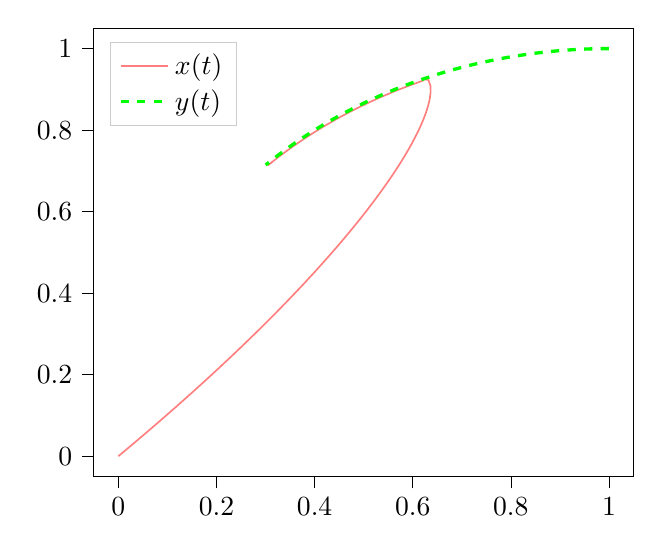
\begin{tikzpicture}

\begin{axis}[
legend cell align={left},
legend style={
  fill opacity=0.8,
  draw opacity=1,
  text opacity=1,
  at={(0.03,0.97)},
  anchor=north west,
  draw=white!80!black
},
tick align=outside,
tick pos=left,
x grid style={white!69.0196078431373!black},
xmin=-0.05, xmax=1.05,
xtick style={color=black},
y grid style={white!69.0196078431373!black},
ymin=-0.05, ymax=1.05,
ytick style={color=black}
]
\addplot [semithick, red, opacity=0.5]
table {%
0 0
0.0105932851190288 0.0106198960414178
0.021159700236 0.02126652698891
0.0316988822130722 0.0319401168028786
0.0422104569586439 0.0426408957383119
0.0526940389199339 0.0533691006111101
0.063149230544578 0.0641249750791759
0.0735756217088786 0.0749087699392946
0.0839727891101328 0.0857207434409194
0.0943402956202228 0.0965611616180674
0.104677689597386 0.10743029864064
0.114984504152788 0.118328437186596
0.125260256368191 0.129255868836524
0.135504446460648 0.140212894492321
0.145716556889743 0.151199824821814
0.155896051402429 0.162216980731347
0.166042374010034 0.173264693868552
0.176154947891387 0.184343307157712
0.18623317421542 0.195453175370385
0.196276430875824 0.206594665734204
0.206284071129573 0.217768158583058
0.216255422130141 0.228974048052206
0.226189783345249 0.240212742822208
0.236086424847735 0.251484666916021
0.245944585466824 0.262790260553995
0.25576347078549 0.27412998107211
0.265542250967865 0.285504303909306
0.275280058398616 0.296913723670478
0.284975985113851 0.308358755272424
0.294629080000491 0.319839935180906
0.304238345737879 0.331357822747954
0.313802735451851 0.342913001659649
0.323321149047308 0.35450608150589
0.33279242918045 0.3661376994851
0.34221535682614 0.377808522258513
0.351588646389225 0.38951924797057
0.360910940300707 0.401270608454232
0.370180803030418 0.413063371642535
0.379396714436786 0.42489834421074
0.388557062361119 0.436776374476913
0.397660134358122 0.448698355592838
0.406704108435419 0.460665229061943
0.415687042651996 0.472677988626568
0.424606863397761 0.484737684573505
0.433461352142544 0.496845428514657
0.442248130401335 0.509002398708968
0.450964642611308 0.521209846002988
0.459608136552474 0.533469100480782
0.468175640864278 0.545781578930001
0.476663939110216 0.558148793250353
0.48506953971549 0.570572359954255
0.493388640940294 0.583054010938084
0.501617089841821 0.595595605737447
0.509750333905566 0.608199145522706
0.517783363668394 0.620866789143687
0.525710644180233 0.633600871597323
0.533526032512506 0.646403925371912
0.541222677652617 0.659278705220098
0.548792897926292 0.672228217033434
0.556228029414238 0.685255751638129
0.563518236447625 0.698364924506905
0.57065227181929 0.711559722584032
0.577617169257636 0.724844559637692
0.584397843028219 0.73822434174943
0.590976557642789 0.751704544632362
0.597332211745117 0.765291304218482
0.603439349177112 0.778991520856151
0.6092667572795 0.792812974293959
0.614775418271778 0.806764438434008
0.619915403195263 0.820855764084858
0.624620946917299 0.835097844281568
0.62880218948818 0.849502230521717
0.632330290465487 0.864079734662894
0.63500785433867 0.878835891932277
0.636501291401439 0.89375519881629
0.63614554409209 0.908731860363251
0.631944396868688 0.922867110567458
0.625929499266278 0.924530136153144
0.622769953808564 0.923630192306444
0.62011865828777 0.921051836867392
0.61397871158503 0.918559919021901
0.609776714095582 0.916617683163057
0.605177239047701 0.914527148052339
0.600499725338173 0.912535706382767
0.595954498228315 0.910554551401068
0.591429392662837 0.908522481361473
0.586888339848174 0.906461894742526
0.582356182099426 0.904385286905881
0.577840487902751 0.902287207448624
0.573335443928958 0.900165031053234
0.568839706082846 0.898020142061739
0.564354775835445 0.895853159303068
0.559881042790697 0.893663816386726
0.555418294919473 0.891452049749428
0.550966593143991 0.889217991261226
0.54652612372493 0.886961721221984
0.542097006328689 0.884683277857244
0.537679334444396 0.882382713150513
0.533273217198133 0.880060088906855
0.528878768681292 0.877715464186126
0.524496098906028 0.875348896596565
0.520125316544535 0.872960445108438
0.515766530865101 0.870550169668123
0.51141985103896 0.868118130568892
0.507085385725658 0.865664388556938
0.502763243241337 0.863189004969141
0.498453531642635 0.860692041702603
0.494156358682207 0.858173561182354
0.489871831788038 0.855633626367367
0.48560005807084 0.853072300755728
0.481341144325069 0.850489648381112
0.477095197023838 0.847885733809705
0.472862322315515 0.845260622139085
0.468642626021641 0.842614378996908
0.464436213634427 0.83994707053915
0.460243190313987 0.837258763448382
0.456063660885681 0.834549524932132
0.45189772983752 0.831819422721224
0.447745501317565 0.829068525068072
0.443607079131315 0.826296900744975
0.439482566739108 0.823504619042395
0.435372067253538 0.82069174976723
0.43127568343688 0.817858363241065
0.427193517698515 0.815004530298416
0.423125672092373 0.812130322284957
0.419072248314384 0.80923581105574
0.41503334769993 0.806321068973394
0.411009071221317 0.803386168906319
0.406999519485247 0.800431184226865
0.403004792730304 0.797456188809494
0.39902499082445 0.794461257028937
0.395060213262523 0.791446463758333
0.391110559163759 0.788411884367356
0.387176127269302 0.785357594720332
0.383257015939745 0.782283671174345
0.379353323152669 0.779190190577322
0.375465146500188 0.776077230266117
0.371592583186516 0.772944868064577
0.367735730025535 0.769793182281592
0.363894683438374 0.766622251709144
0.360069539450996 0.763432155620331
0.356260393691802 0.760222973767389
0.352467341389237 0.756994786379699
0.348690477369413 0.753747674161775
0.344929896053731 0.750481718291256
0.34118569145653 0.747197000416866
0.33745795718273 0.743893602656383
0.333746786425492 0.740571607594578
0.330052271963894 0.737231098281154
0.326374506160603 0.73387215822867
0.322713580959573 0.730494871410454
0.319069587883744 0.727099322258498
0.315442618032753 0.723685595661356
0.311832762080657 0.720253776962015
0.308240110273667 0.716803951955762
0.304664752427892 0.713336206888044
};
\addlegendentry{$x(t)$}
\addplot [very thick, green, dashed]
table {%
1 1
0.995000020833306 0.999987500026042
0.990000166665831 0.999950000416665
0.985000562493669 0.999887502109359
0.980001333306663 0.999800006666578
0.975002604085282 0.999687516275703
0.970004499797498 0.999550033748987
0.965007145395656 0.999387562523488
0.960010665813357 0.999200106660978
0.95501518596233 0.998987670847842
0.950020830729311 0.998750260394966
0.94502772497292 0.998487881237598
0.940035993520542 0.998200539935204
0.935045761165203 0.997888243671301
0.930057152662452 0.997551000253279
0.925070292727241 0.997188818112207
0.92008530603081 0.996801706302619
0.915102317197565 0.99638967450229
0.910121450801969 0.995952733011993
0.905142831365422 0.995490892755244
0.90016658335315 0.995004165278025
0.895192831171095 0.994492562748496
0.890221699162801 0.993956097956696
0.885253311606311 0.993394784314214
0.880287792711055 0.992808635853865
0.875325266614745 0.992197667229327
0.870365857380277 0.991561893714786
0.865409688992622 0.990901331204546
0.860456885355733 0.990215996212635
0.855507570289442 0.989505905872392
0.850561867526368 0.98877107793604
0.845619900708823 0.988011530774237
0.840681793385719 0.987227283375624
0.835747669009483 0.986418355346345
0.830817650932967 0.985584766909558
0.825891862406366 0.98472653890493
0.820970426574137 0.983843692788118
0.816053466471919 0.982936250630228
0.811141105023458 0.982004235117266
0.806233465037536 0.981047669549573
0.801330669204896 0.980066577841237
0.796432840095178 0.9790609845195
0.791540100153855 0.978030914724143
0.786652571699171 0.976976394206857
0.781770376919083 0.9758974493306
0.776893637868206 0.974794107068938
0.772022476464762 0.973666395005369
0.767157014487533 0.972514341332637
0.762297373572814 0.971337974852023
0.757443675211375 0.970137324972629
0.752596040745423 0.968912421710638
0.747754591365567 0.967663295688568
0.742919448107789 0.966389978134506
0.738090731850419 0.965092500881323
0.733268563311111 0.963770896365883
0.728453063043828 0.96242519762823
0.723644351435826 0.961055438310762
0.718842548704645 0.959661652657392
0.714047774895102 0.958243875512688
0.709260149876294 0.956802142321004
0.704479793338596 0.955336489125596
0.699706824790673 0.953846952567717
0.69494136355649 0.952333569885703
0.69018352877233 0.950796378914042
0.685433439383814 0.94923541808243
0.68069121414293 0.947650726414804
0.675956971605061 0.946042343528375
0.671230830126025 0.944410309632631
0.666512907859113 0.942754665528334
0.661803322752135 0.9410754526065
0.657102192544474 0.939372712847366
0.65240963476414 0.937646488819336
0.647725766724833 0.935896823677921
0.643050705523011 0.934123761164659
0.638384568034959 0.932327345606019
0.633727470913873 0.930507621912299
0.629079530586937 0.928664635576494
0.624440863252417 0.926798432673169
0.619811584876756 0.924909059857296
0.615191811191671 0.9229965643631
0.610581657691265 0.921060994002868
0.605981239629134 0.919102397165757
0.60139067201549 0.917120822816587
0.596810069614286 0.915116320494613
0.592239546940341 0.913088940312289
0.587679218256486 0.911038732954014
0.583129197570698 0.908965749674865
0.57858959863326 0.906870042299316
0.574060534933908 0.904751663219942
0.569542119698997 0.902610665396111
0.565034465888675 0.900447102352655
0.560537686194051 0.898261028178539
0.556051893034384 0.896052497525502
0.551577198554268 0.893821565606697
0.547113714620833 0.891568288195305
0.542661552820945 0.889292721623144
0.538220824458416 0.886994922779259
0.533791640551226 0.884674949108503
0.529374111828739 0.882332858610096
0.524968348728946 0.879968709836178
0.520574461395693 0.877582561890346
0.516192559675934 0.875174474426174
0.511822753116986 0.872744507645723
0.507465150963784 0.870292722298037
0.503119862156155 0.867819179677621
0.498786995326093 0.865323941622912
0.494466658795043 0.862807070514731
0.490158960571193 0.860268629274725
0.485864008346775 0.857708681363793
0.48158190949537 0.855127290780499
0.477312771069227 0.852524522059473
0.473056699796584 0.849900440269799
0.468813802079001 0.847255111013383
0.4645841839887 0.844588600423319
0.460367951265913 0.841900975162234
0.456165209316239 0.839192302420619
0.451976063208007 0.836462649915151
0.447800617669652 0.833712085887001
0.443638977087095 0.830940679100126
0.439491245501134 0.828148498839552
0.435357526604842 0.82533561490964
0.431237923740976 0.822502097632341
0.427132539899394 0.81964801784544
0.423041477714478 0.816773446900783
0.418964839462568 0.813878456662493
0.414902727059411 0.810963119505177
0.410855242057602 0.80802750831211
0.406822485644058 0.80507169647342
0.402804558637478 0.802095757884249
0.398801561485828 0.799099766942907
0.394813594263829 0.796083798549011
0.390840756670453 0.793047928101614
0.386883148026433 0.789992231497319
0.382940867271779 0.786916785128382
0.379014012963305 0.783821665880802
0.375102683272164 0.780706951132399
0.371206975981395 0.777572718750879
0.367326988483476 0.774419047091889
0.363462817777894 0.771246014997057
0.359614560468714 0.768053701792018
0.355782312762169 0.764842187284437
0.351966170464252 0.76161155176201
0.348166228978321 0.758361875990455
0.344382583302717 0.755093241211499
0.340615328028383 0.751805729140841
0.336864557336506 0.74849942196611
0.333130364996157 0.745174402344815
0.32941284436195 0.741830753402272
0.325712088371708 0.738468558729531
0.322028189544138 0.735087902381284
0.318361239976518 0.731688868873762
0.314711331342396 0.728271543182628
0.311078554889299 0.724836010740845
0.307463001436448 0.721382357436546
0.303864761372492 0.717910669610882
0.300283924653244 0.714421034055869
};
\addlegendentry{$y(t)$}
\end{axis}

\end{tikzpicture}

    \end{center}
    В такому випадку $P$ наздожене $E$ в момент $T \approx 0.385$ у точці $\begin{pmatrix}
        0.625 \\ 0.925
    \end{pmatrix}$.
\end{example}